\mode*
\begin{frame}[label=investigador]
  \investigadorTime
  \frametitle{Viabilidad}
  \framesubtitle{Experiencia del investigador y coherencia}
  \quad\hspace{-0.8cm}\vspace{-0.5cm}
  \begin{columns}[T,totalwidth=0.97\textwidth]
    \small
    \begin{column}{0.55\textwidth}\setbeamercovered{transparent}
      \begin{itemize}
      \item<1-|alert@1|uncover@1-11> Algunos trabajos del investigador
        \only<1->{
          \begin{enumerate}\scriptsize\setbeamercovered{transparent}
          \item<2-|alert@2|uncover@2-3> Desarrollo de librerias en C/C++ y MATLAB
          \item<4-|alert@4|uncover@4-5> An\'alisis de caminadores
          \item<6-|alert@6|uncover@6-7> Construcci\'on de plataformas rob\'oticas
          \item<8-|alert@8|uncover@8-9> Optimizaci\'on morfol\'ogica
          \item<10-|alert@10|uncover@10-11> Optimizaci\'on topol\'ogica
          \end{enumerate}
        }
      \end{itemize}
    \end{column}
    \begin{column}{0.4\textwidth}
      \parbox[c][7cm][c]{4.0cm}{
        \only<3>{
          \scriptsize
          \begin{center}%P1(120,360),P2(1110,530)
            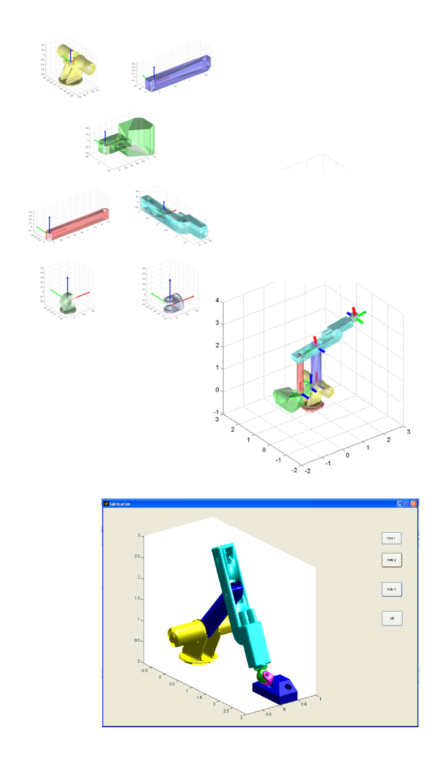
\includegraphics[height=7cm]{../images/SomeThingsByMe_1.png}
          \end{center}
        }
        \only<5>{
          \scriptsize
          \begin{center}%P1(120,360),P2(1110,530)
            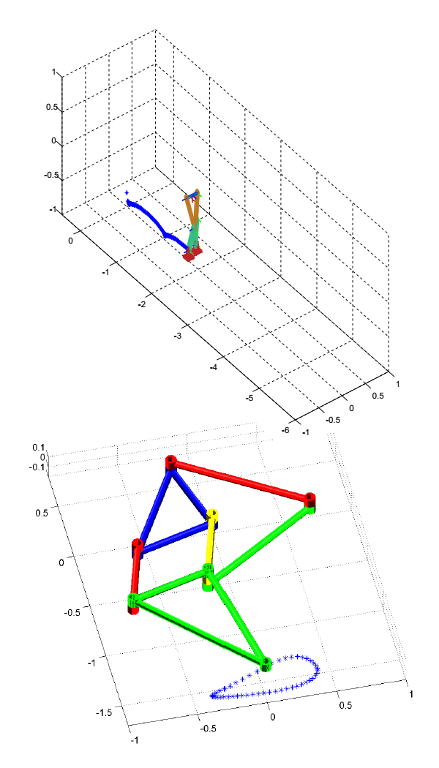
\includegraphics[height=7cm]{../images/SomeThingsByMe_2.png}
          \end{center}
        }
        \only<7>{
          \scriptsize
          \begin{center}%P1(120,360),P2(1110,530)
            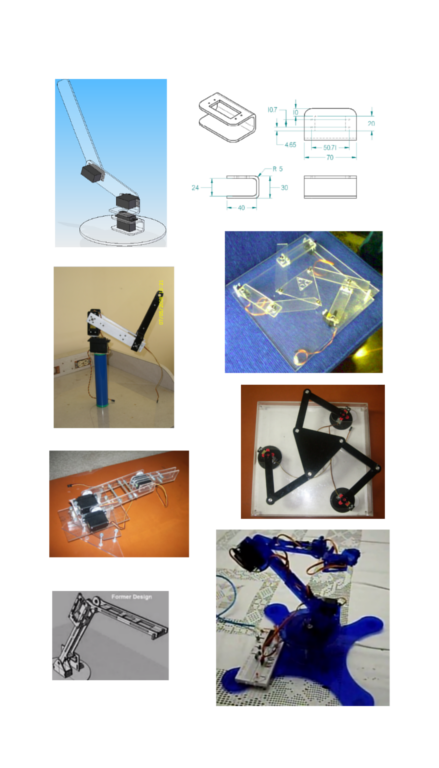
\includegraphics[height=7cm]{../images/SomeThingsByMe_3.png}
          \end{center}
        }
        \only<9>{
          \scriptsize
          \begin{center}%P1(120,360),P2(1110,530)
            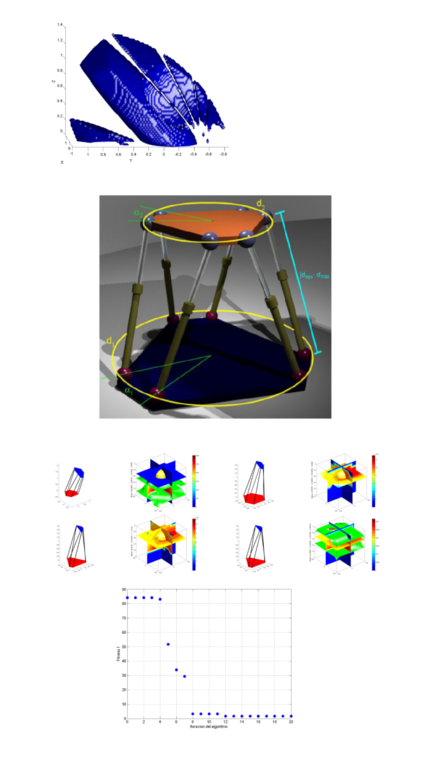
\includegraphics[height=7cm]{../images/SomeThingsByMe_4.png}
          \end{center}
        }
        \only<11>{
          \scriptsize
          \begin{center}%P1(120,360),P2(1110,530)
            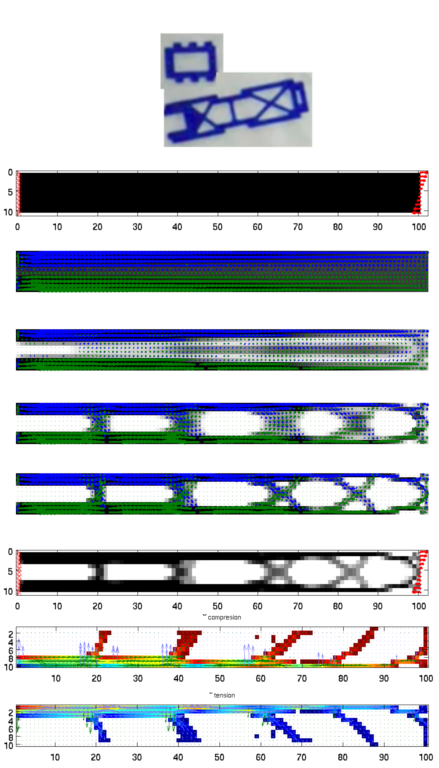
\includegraphics[height=7cm]{../images/SomeThingsByMe_5.png}
          \end{center}
        }
      }
    \end{column}
  \end{columns}
\end{frame}
